\section{Metodología}



En esta sección se presenta como determinar la precisión $(R^{2})$ de modelos con la técnica de regresión lineal con estimadores Bootstrap robustos. Con modelos Exactos-Precisos (EP) y Exactos-Imprecisos (EI) con su muestra de estimaciones de $R^{2}$ respectivo para cada caso: Normalidad - Varianza Constante (NVC), No normalidad - Varianza Constante (NNVC), Normalidad - Varianza Distinta (NVD) y No normalidad - Varianza Distinta (NNVD). Utilizando diversos esquemas de remuestreo Bootstrap para la construir un intervalo de confianza para la $R^{2}$.\\


Para ello se simularon apriori 2,500 modelos para tipos de modelo Exacto-Preciso (EP) y Exacto-Impreciso (EI) con su muestra de estimaciones de $R^{2}$ respectivo para cada caso: Normalidad - Varianza Constante (NVC), No normalidad - Varianza Constante (NNVC), Normalidad - Varianza Distinta (NVD) y No normalidad - Varianza Distinta (NNVD), divididas en 5 replicas y por tamaño de muestra  = 







 una muestra de tamaño 2500 estimaciones de $R^{2}$ con los diferentes esquemas de remuestreo Bootstrap propuestos en Rana et al. (2012), tomando en consideración cuando se cumplan los supuestos de normalidad y/o igualdad de varianzas en el modelo de regresión lineal entre los valores reales $( y_{i} )$  y los simulados $( z_{i} )$ por el modelo matemático a evaluar. Posteriormente se determinarán intervalos de confianza Bootstrap para la  $R^{2}$.
\vspace{.5cm}



Cuando se cumplan los supuestos de normalidad e igualdad de varianzas, en el esquema de Bootstrap se utilizarán los estimadores de mínimos cuadrados para el cálculo de $R^{2}$ y se usarán los residuales del modelo de regresión para generar nuevas observaciones $ y_{i}^{*} $ y de esta manera obtener las estimaciones Bootstrap para $R^{2}$  con el modelo de regresión entre $ y_{i}^{*} $  y  $ z_{i} $. Posteriormente, para evaluar la precisión, se determinará la estimación de $R^{2}$ con intervalos de confianza Bootstrap con los métodos: Percentil y Percentil con sesgo corregido acelerado (BCa).
\vspace{.5cm}

Cuando no se cumplan los supuestos de normalidad y/o igualdad de varianzas, en el esquema de Bootstrap se utilizará el MM-Estimador robusto de la pendiente y se ponderarán los residuales del modelo de regresión para generar nuevas observaciones $ y_{i}^{*} $ y de esta forma obtener las estimaciones Bootstrap para $R^{2}$ con el modelo de regresión entre $ y_{i}^{*} $  y  $ z_{i} $. Posteriormente,
para evaluar la precisión, se determinará la estimación de $R^{2}$ con un intervalo de confianza Bootstrap con los métodos:  Percentil y BCa.
\vspace{.5cm}


Para evaluar la eficacia de la metodología propuesta en los objetivos específicos 2 y 3, se simularán modelos con la propuesta de Febles (2014) y las mejoras establecidas en Zacarías (2023); para ello se simularán modelos considerando los siguientes factores: Precisión (EP, EI), tamaño de muestra $(n=10,15,20,25,30,35)$, y supuesto (N-VC, N-VD, NN-VC, NN-VD); dando un total de 48 escenarios posibles para los modelos simulados. Para cada escenario se simularán 500 modelos, por lo que en total se tendrán 24,000 modelos simulados. Para los modelos EP se utilizarán números aleatorios para $R^{2}$  entre 0.9 y 0.99; y para los modelos EI se utilizarán números aleatorios para  $R^{2}$   entre 0.3 y 0.6. Para cada modelo simulado, se guardará el valor de $R^{2}$  que fue seleccionado para su simulación, esto con el propósito de evaluar la eficacia de los intervalos Bootstrap.
\vspace{.5cm}


Para determinar la eficacia de los intervalos de confianza Bootstrap (ICB) en la evaluación de la precisión para los diferentes tipos de modelos (EP, EI), se tomará como criterio que el intervalo contenga al valor a priori $R^{2}$ que generó al modelo simulado correspondiente; y en caso de que éste lo contenga se determinará el ancho del ICB. Tanto para los modelos simulados EP y EI, se determinará el porcentaje de las veces en que el ICB contuvo al valor a priori $R^{2}$ correspondiente.
\vspace{.5cm}

Para determinar el tipo de ICB más eficaz en la evaluación de la precisión cuando los modelos simulados (EP, EI) cumplen el supuesto N-VC, se utilizará el ANOVA para un arreglo factorial con dos factores (Montgomery, 2017): tamaño de muestra y tipo de ICB.
Para determinar el tipo de ICB más eficaz en la evaluación de la precisión cuando los modelos simulados (EP, EI) no cumplen los supuestos, se utilizará el ANOVA para un arreglo factorial con tres factores (Montgomery, 2017): tamaño de muestra, tipo de ICB y supuestos (N-VD, NN-VC, NN-VD).
En caso de diferencias estadísticas significativas, se utilizará la comparación múltiple de Tukey (Montgomery, 2017).
Las pruebas estadísticas se considerarán significativas cuando $p \leq 0.05 $.
\vspace{.5cm}

El estudio de simulación y la evaluación de la precisión de los ICB se implementará en el lenguaje R (R Core Team, 2023).



\vspace{1.5cm}
\subsection{Método para evaluar la precisión de un modelo}

Desarrollar la metodología para medir la precisión de un modelo con la técnica de regresión lineal por medio de intervalos de confianza basado en diferentes esquemas de remuestreo Bootstrap. 
%aqui el esquema

\begin{figure}[ht] 
	\centering 
	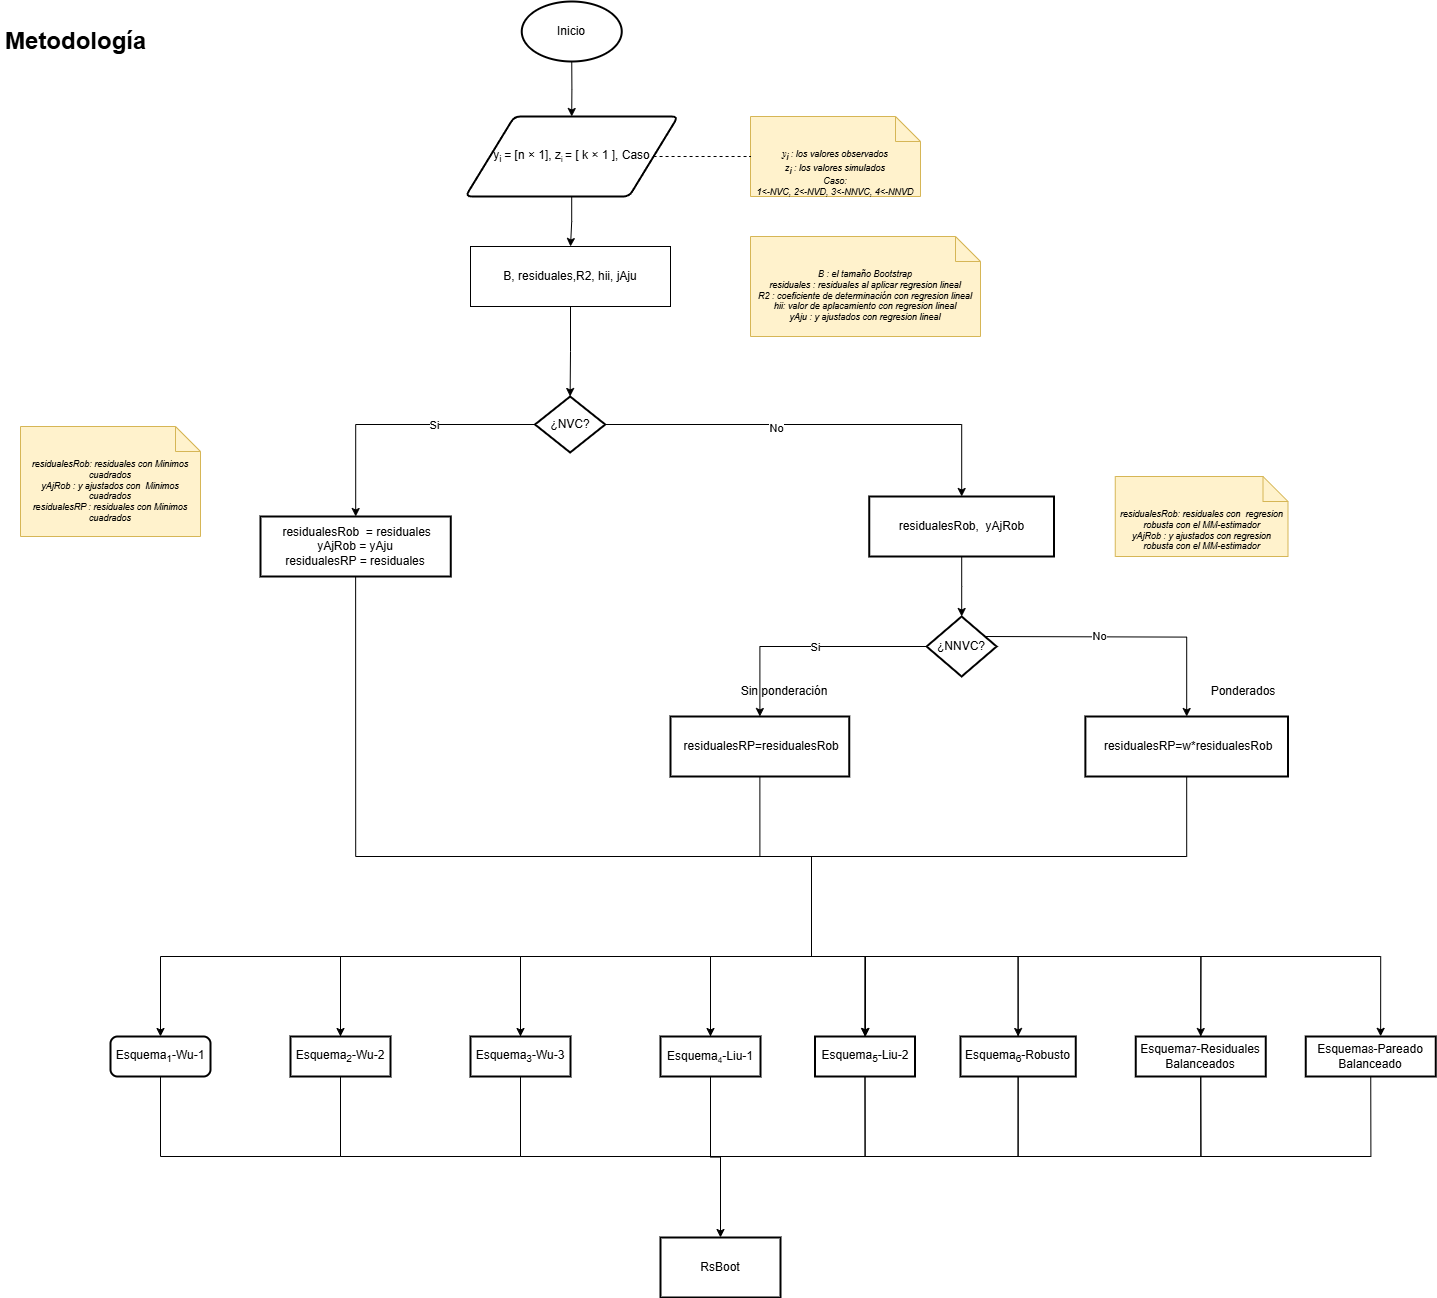
\includegraphics[width=0.98\linewidth]{img/metodologia.png} 
	\caption{Algoritmo para los diferentes esquemas Bootstrap.} 
\end{figure}




	\vspace{1.5cm}
	\subsection{Precisión de modelos que cumplen el supuesto de normalidad y varianza constante}
	 Determinar la precisión de un modelo cuando se cumplan los supuestos de normalidad y varianza constante.
	 \vspace{1.5cm}
	 
	 
	 
	 
	 
	 \subsection{Precisión de modelos que no cumplen el supuesto de normalidad y/o varianza constante}
	 Determinar la precisión de un modelo cuando no se cumplan los supuestos de normalidad y/o varianza constante.
	 \vspace{1.5cm}
	 	 
	 	 
	 \subsection{Estudio de simulación para la evaluación de la propuesta}
	 \vspace{1.5cm}
	
	 \subsubsection{Simulación de modelo}
	 Simular modelos exactos-precisos (EP) y modelos exactos-imprecisos (EI) mediante la propuesta de Febles (2014) y Zacarías (2023); cuando se cumplan o no los supuestos de normalidad e igualdad de varianzas.
	 
	 %aqui va el diagrama
	 Diseñar e implementar un estudio de simulación para evaluar la eficacia de la metodología propuesta.
	 	 \vspace{1.5cm}
	 	 
	 	 
	 	 
	 	 
\subsection{Análisis estadísticos}
Para cada supuesto (NVC, NNVC, NVD, NNVD) se utilizó ANOVA en un arreglo factorial de tres factores seguido de la comparación múltiple de Tukey (Montgomery, 2017), para determinar el comportamiento de la eficacia de dos ICB en la evaluación de la precisión, bajo ocho esquemas de remuestreo, seis tamaños de muestra y dos tipos de modelo. Cabe señalar que, en cuatro de los ocho análisis de varianza realizados se eliminaron valores atípicos para el logro del cumplimiento de los supuestos del ANOVA.
Las pruebas estadísticas se consideraron significativas cuando  y se utilizó el paquete estadístico STATGRAPHICS Centurion 19 (Statgraphics, 2024).




